% LINGI2251
% Development methods
\documentclass[11pt, a4paper]{article}
\usepackage[utf8]{inputenc}
\usepackage[UKenglish]{babel}
\usepackage{graphicx}				% Use pdf, png, jpg, or eps§ with pdflatex; use eps in DVI mode
\usepackage{xcolor}
\usepackage{listings}
\usepackage{hyperref}
\usepackage{array}
\usepackage{longtable}
\usepackage{multirow}
\usepackage[babel=true]{csquotes}


\usepackage[T1]{fontenc}

\lstset{%
	basicstyle=\ttfamily\footnotesize,
	commentstyle=\color{green!90!black},
	frame=single,
	keywordstyle=\bfseries\color{blue},
	language=python,
	numberstyle=\color{gray},
%	tabsize=2,
}


\hypersetup{%
	colorlinks=true,
	linkcolor=blue,
	urlcolor=blue
}


\newcommand{\tbf}[1]{\textbf{#1}}
\newcommand{\tit}[1]{\textit{#1}}

\newcommand{\data}[1]{\textit{#1}}
\newcommand{\state}[1]{\textsf{#1}}



\def\blurb{\textsc{Université catholique de Louvain\\
  École polytechnique de Louvain\\
  Pôle d'ingénierie informatique}}
\def\clap#1{\hbox to 0pt{\hss #1\hss}}%
\def\ligne#1{%
  \hbox to \hsize{%
    \vbox{\centering #1}}}%
\def\haut#1#2#3{%
  \hbox to \hsize{%
    \rlap{\vtop{\raggedright #1}}%
    \hss
    \clap{\vbox{\vfill\centering #2\vfill}}%
    \hss
    \llap{\vtop{\raggedleft #3}}}}%
\begin{document}

\begin{titlepage}
\thispagestyle{empty}\vbox to 1\vsize{%
  \vss
  \vbox to 1\vsize{%
    \haut{\raisebox{-2mm}{
\includegraphics[width=2.5cm]{logo_epl.jpg}}}{\blurb}{\raisebox{-5mm}{
\includegraphics[scale=0.20]{ingi_logo}}}
    \vfill
    \ligne{\Huge \textbf{\textsc{LINGI2251}}}
     \vspace{5mm}
    \ligne{\huge \textbf{\textsc{Development methods}}}
     \vspace{15mm}
    \ligne{\Large \textbf{\textsc{Assignment 2: The Dinoco GSCS}}}
    \vspace{5mm}
    \ligne{\large{\textsc{April 20, 2015}}}
    \vfill
    \vspace{5mm}
    \ligne{%
         \textsc{Professor\\Charles Pecheur}
      }
      \vspace{10mm}
    }%
    \ligne{%
         \textsc{Michael Heraly\\Thibault Gerondal}
      }
      \vspace{5mm}
  \vss
  }
\end{titlepage}



\newpage


\section{Architectural Design}
\subsection{Hierarchical decomposition}

\begin{center}
\centerline{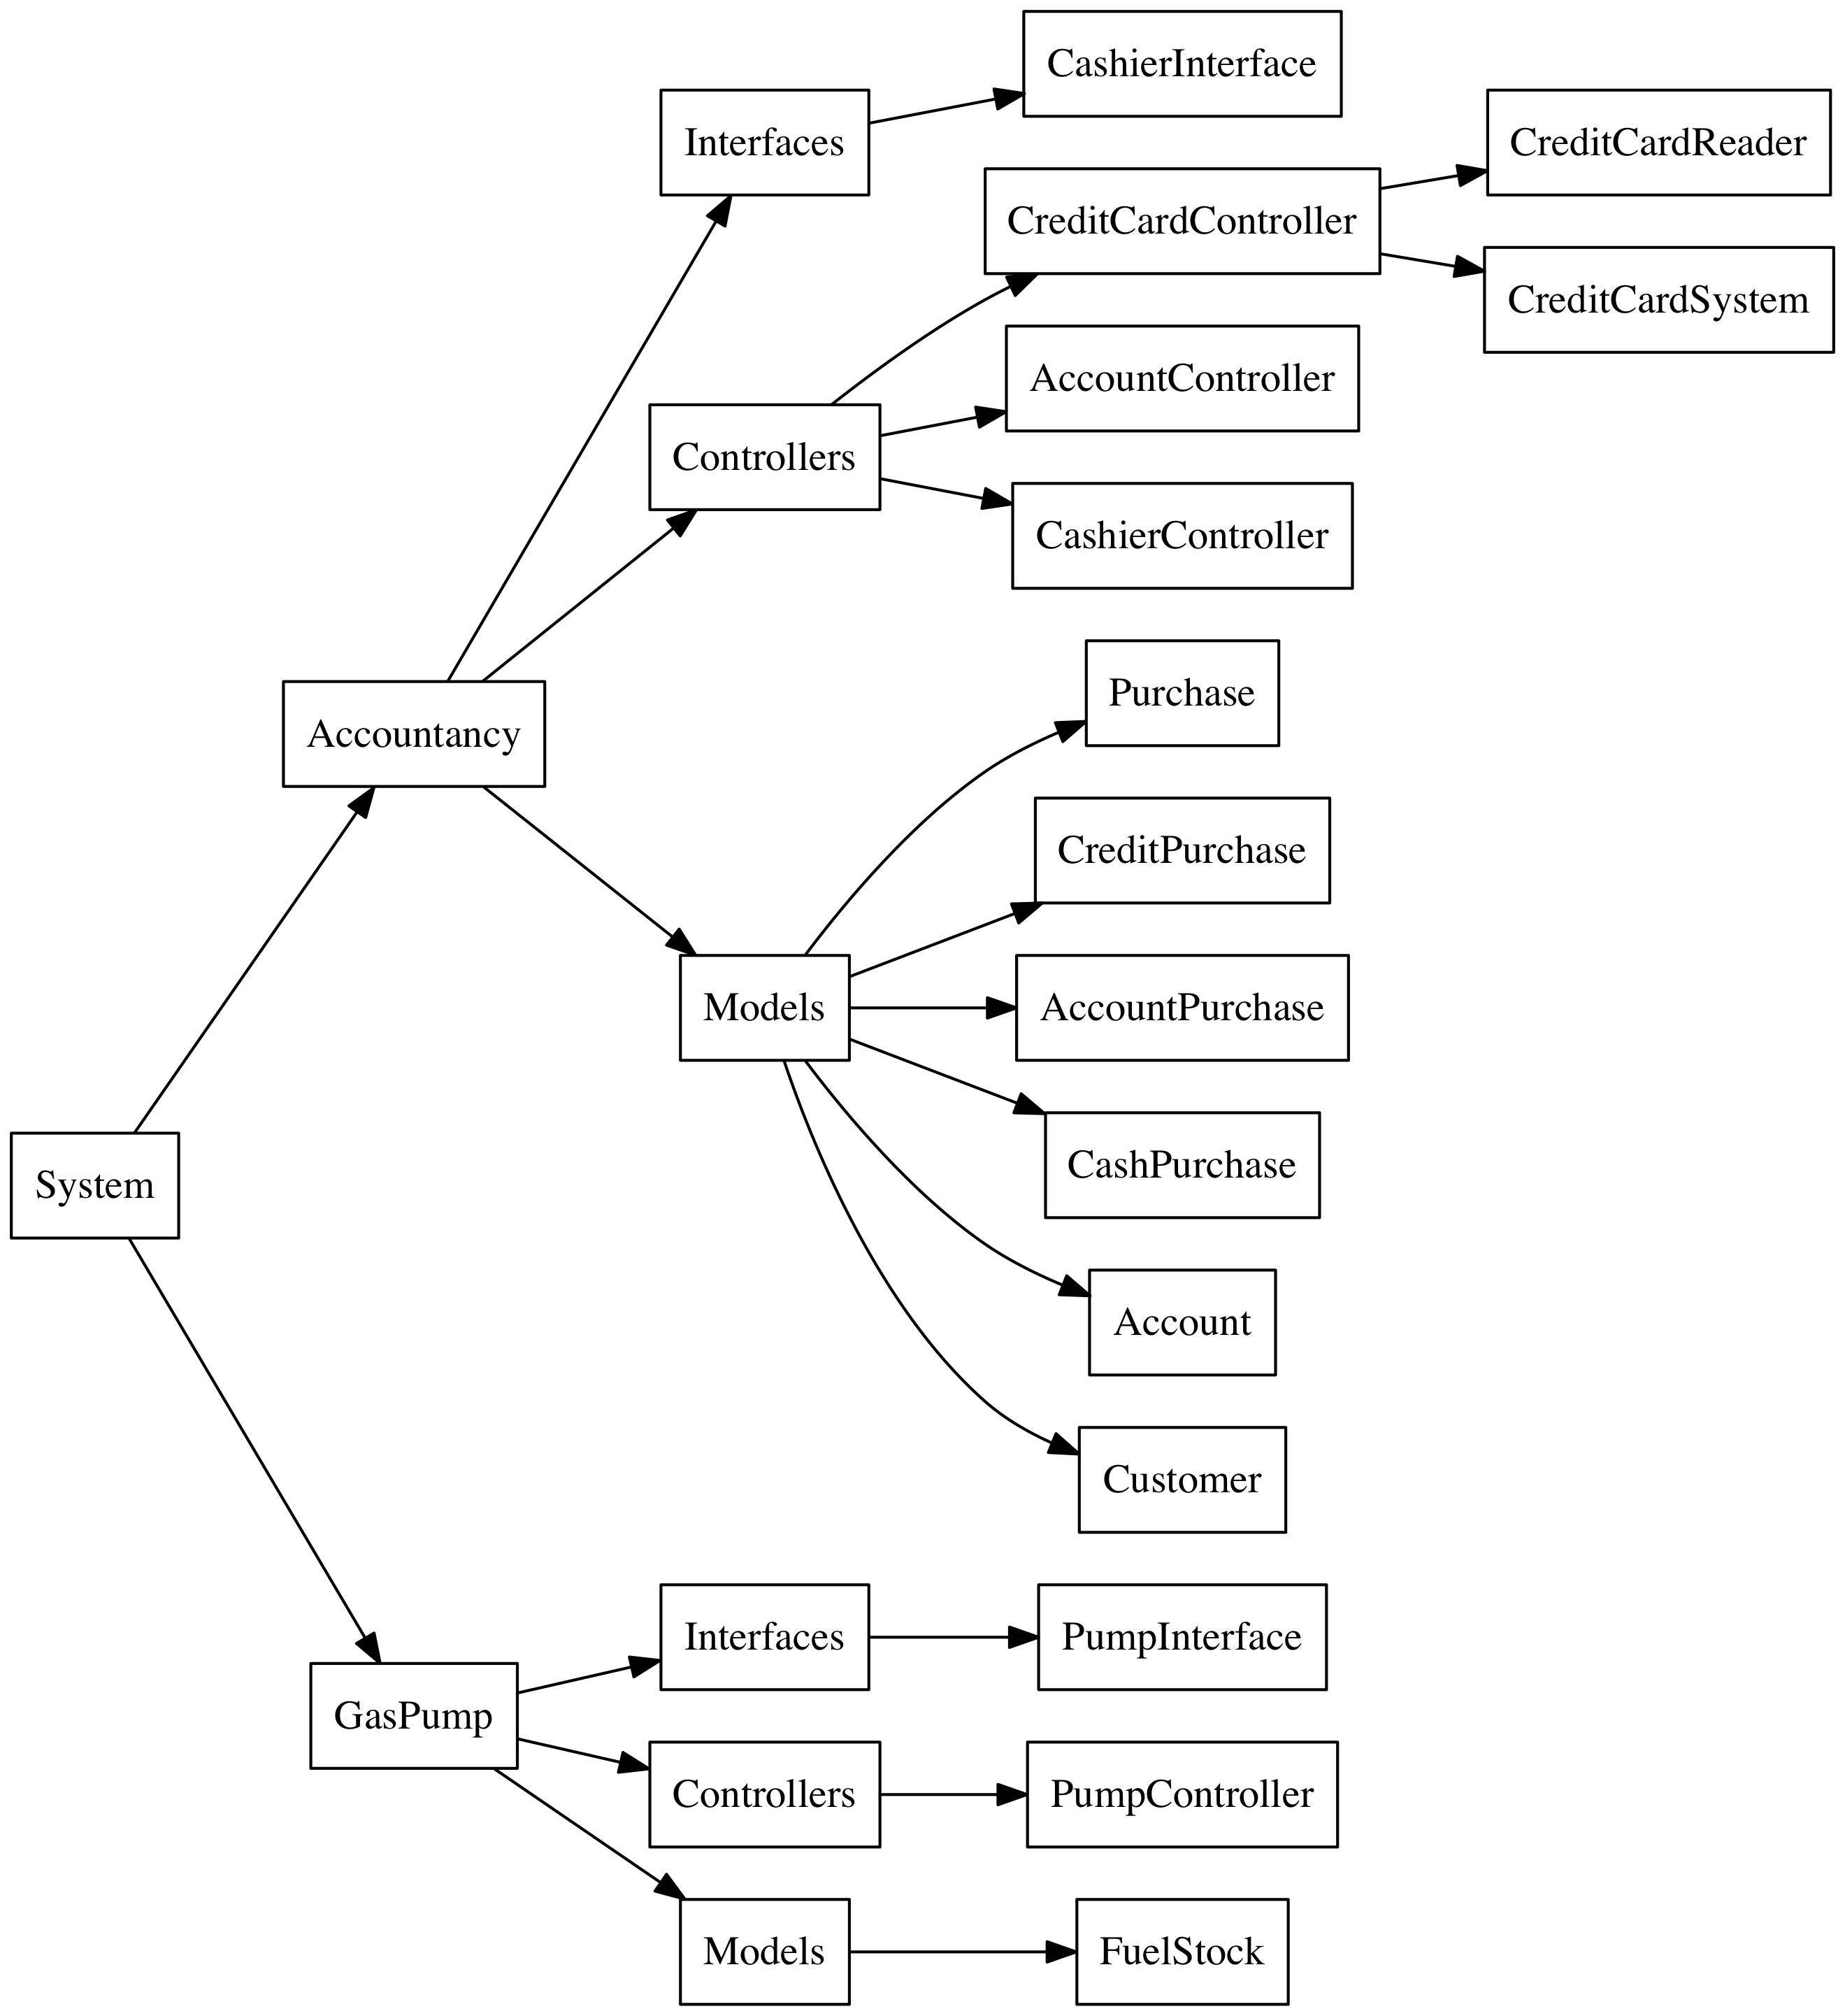
\includegraphics[width=1.3\textwidth]{hierarchical.png}}
\end{center}

\subsection{Roles and interactions}

Our system is composed of two parts : ``Accountancy'' and ``Gas Pump''. The first one is related to accounting. And the second one is about the logistic of the gas pump. This hierarchy allows to easily extend the activities of \textbf{Dinoco GSCS}.\\




In each of these two sections, we defined three components : ``Interfaces'', ``Controllers'', ``Storages''.\\


Here are the descriptions of the system components :
\begin{description}
\item[CashierInterface] is responsible for displaying the graphical user interface to the cashier.
\item[CashierController] is responsible for manipulating every . 
\end{description}

\end{document}
